\documentclass[12pt,a4paper]{extarticle}
\usepackage{ascmac, amsmath,amssymb, url, pifont}
%\usepackage{bm}
\usepackage[at]{easylist}
\usepackage[dvipdfmx]{graphicx, xcolor} % 枠組み
\usepackage{tikz}
\usepackage[framemethod=tikz]{mdframed}
\usepackage[top=10truemm,bottom=10truemm,left=20truemm,right=20truemm]{geometry}
\renewcommand{\baselinestretch}{1.5}
\pagestyle{empty}
\global\mdfdefinestyle{exampledefault}{%
	middlelinewidth=1pt,%
	leftmargin=1cm,rightmargin=1cm}
\makeatletter 
\def\section{\@startsection {section}{1}{\z@}{-3.5ex plus -1ex minus -.2ex}{2.3 ex plus .2ex}{\large\bf}} % change section style
\def\subsection{\@startsection {subsection}{1}{\z@}{-3.5ex plus -1ex minus -.2ex}{2.3 ex plus .2ex}{\normalsize\bf}}
\makeatother

\newcommand{\point}[1]
{\textbf{\textcolor{magenta}{#1}}}
\newcommand{\obs}[1]
{\textbf{\textcolor{violet}{#1}}}
\newcommand{\rec}[1]
{\textbf{\textcolor{orange}{#1}}}
%#######*****#######*****#######*****#######***
\begin{document} 

\noindent\textbf{\Large{函南毎木調査マニュアル} \small{(140809 瓜生作成) ver.0.1}}\\

\subsection*{プロット設計}

函南原生林内の600mから800mまでの範囲に、100m間隔でプロットが設置されている。\textbf{各プロットの面積は600m 2.0ha、700m 1.1ha、800m 1.1ha}である。すべての\textbf{プロットは10m $\times$ 10mのメッシュに分割}されており、アルファベットと数字からなるメッシュ番号が与えられている(e.g. \textbf{A14})。

\begin{figure}[tb]
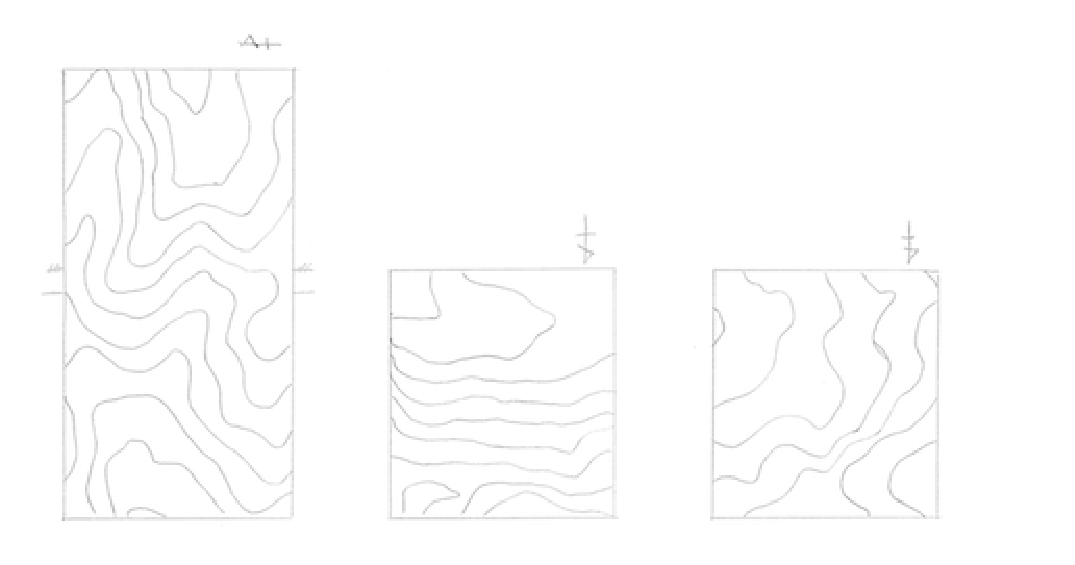
\includegraphics[]{../Images/plotmap.eps}
\label{函南原生林毎木プロットの等高線図。左から600m、700m、800mのプロット}
\end{figure}

\subsection*{作業内容}

作業は基本的に\rec{測定係}2名と\obs{記録係}1名での3名一組で行う。2組で調査を行う場合は、並行して調査を行うようにし、各組で1列を担当するようにする。

\subsubsection*{手順}

一例として。各自が調査しやすい手順で行うのが望ましい。

\begin{easylist}
@ メッシュ内に含まれるタグ番号がついている個体の記録・測定
@@ \textbf{\colorbox[HTML]{00FF80}{%
調査をした個体にはチョークで印}}をつけておくと測定の重複を防ぐことができる
@@ ササの多いメッシュでは個体を探すのが大変...
@@@ 対象個体が\textbf{どうしても}見つからない場合(枯死している可能性もあるので倒れた幹なども確認)は欠測として記録する。
@ メッシュ内でタグ番号がついていない\point{新規個体(直径5cm以上)}の記録・測定
@@ 基準となる5cmの大きさをあらかじめ把握しておくと良い\\\rule{5cm}{.8pt}←これが5cmの長さ(大体親指の長さくらい)
\end{easylist}


\subsubsection*{計測項目}

\begin{easylist}[enumerate]
@ 胸高周囲長(\point{GBH$_{14}$}): 地上高1.3m... おおよそ自分の胸の高さでの樹木の幹周囲
@ 萌芽の有無(\point{Spr$_{14}$}): 地際30cm以下から発生しているものを萌芽とする。\textbf{萌芽幹を持つものには1}、萌芽していないものには0を与える
@ 光環境の評価(\point{CPI$_{14}$}): 
@ 生死の判定(\point{LD$_{14}$}): 
@@ 死亡要因は\point{Note}欄に記録する。死亡要因としては\textcolor{cyan}{枯死、幹折れ、根返り}がある
\end{easylist}

\begin{figure}
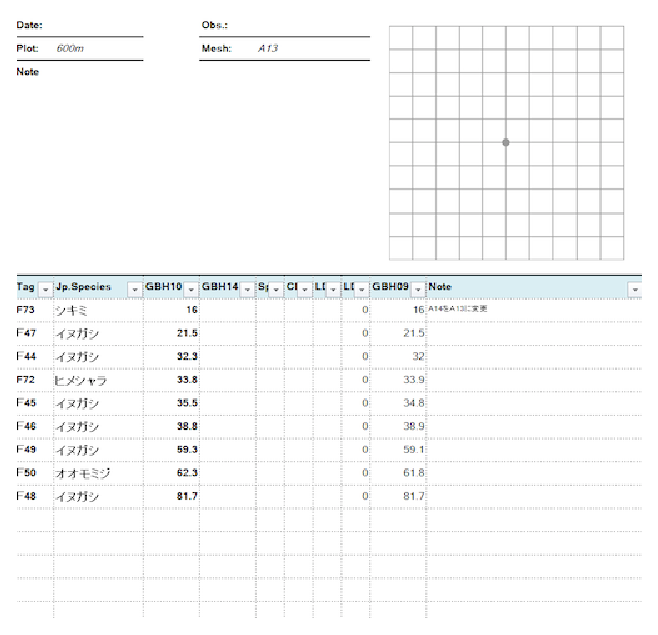
\includegraphics[]{../Images/datasheet-sample.eps}
\end{figure}


\subsection*{出現種}

標高の違いを反映し、プロットごとに出現種は異なるが、次のものがこれまでの調査で出現している。

\begin{mdframed}[style=exampledefault,roundcorner=5]\small{
ブナ、アカガシ。。。
}\end{mdframed}

\newpage
%#######*****#######*****#######*****#######***



\end{document} 